Motyw graficzny systemu można modyfikować lub skorzystać z gotowców. Domyślnie w Ubuntu zainstalowane są trzy motywy: Ambiance (ciemny), Radiance (jasny) i High Contrast (wysoki kontrast). Zmiana motywu graficznego odbywa się poprzez \menu{{Ustawienia systemu}>{Wygląd}>{Motyw}}.

Aby pobrać i zainstalować nowy motyw, otwórz stronę \href{http://gnome-look.org/}{Gnome-Look.org} i z panelu po lewej stronie wybierz dział ,,GTK 3.x''. Wybierz interesujący cię motyw i kliknij przycisk \textcolor{ubuntu_orange}{download}. Otwórz pobrany plik w menedżerze archiwów File-Roller. Zobaczysz okno podobne do tego:

\begin{center}
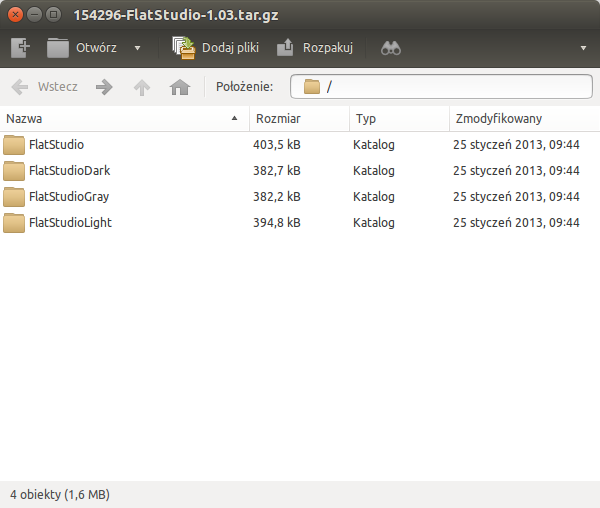
\includegraphics[width=\linewidth]{images/programy_fileRoller.png}
\end{center}

Większość motywów pakowana jest w paczki po kilka sztuk różniących się kolorystyką. Wybierz jeden (lub wszystkie) i kliknij przycisk \textcolor{ubuntu_orange}{Rozpakuj}. W otwartym oknie musisz wskazać gdzie mają zostać wypakowane pliki. Motywy graficzne przechowywane są w katalogu domowym, w podkatalogu .themes. Nie masz jeszcze tego katalogu, więc upewnij się, że masz otwarty katalog domowy, a następnie kliknij przycisk \textcolor{ubuntu_orange}{Utwórz katalog}, znajdujący się w prawym górnym rogu okna. Jako nazwę katalogu podaj .themes (z kropką na początku). Utworzysz w ten sposób ukryty katalog, przeznaczony na motywy graficzne. Wypakuj zawartość pobranego z internetu pliku do nowo utworzonego katalogu.

Teraz należy poinformować system, że ma używać nowego motywu graficznego. Uruchom \textcolor{ubuntu_orange}{Unity Tweak Tool}, a następnie z wiersza \textcolor{ubuntu_orange}{Appearance} wybierz \textcolor{ubuntu_orange}{Theme}. Na wyświetlonej liście wymienione są wszystkie motywy zainstalowane w systemie. Kliknięcie nazwy motywu automatycznie wprowadza zmiany.
